point cloud\chapter{Methodology}
\label{ch:intro}

\section{System Overview}

The architecture overview and the complete step-by-step algorithm flow of the proposed localization system are shown in Figure \ref{fig:diagram-map-basedlocalization} and Algorithm \ref{alg:localization-system}. The input of the system includes the raw online point-cloud, raw IMU data as well as the prior map , and output real-time accurate 6 DOF pose.	

The system can be divided in to different modules:


\begin{enumerate}
	\item Scan Pre-Processing: Performs a series of point cloud processing steps to filter and extract relevant features from the raw LiDAR data.
	
	\item LIDAR-INERTIA Odometry - Estimates high-frequency odometry by fusing raw IMU data and LiDAR scans. The resulting odometry is added as a local constraint (odom factor) to the factor graph.
	
	\item Dynamic Local Map Loader: Generates a local map around the robot’s current pose within a specified radius from the prior map.
	
	
	\item Scan-to-Map Matching: Aligns the current LiDAR scan with the local map to estimate the robot's pose in the prior map. The estimated pose is added as a prior constraint (map factor) to the factor graph.
	
	\item Sliding Window Factor Graph Optimizer:Fuses odometry and map constraints within a sliding window to optimize and output a real-time, accurate 6-DoF pose.
	
	
\end{enumerate}

\begin{figure}
    \centering
    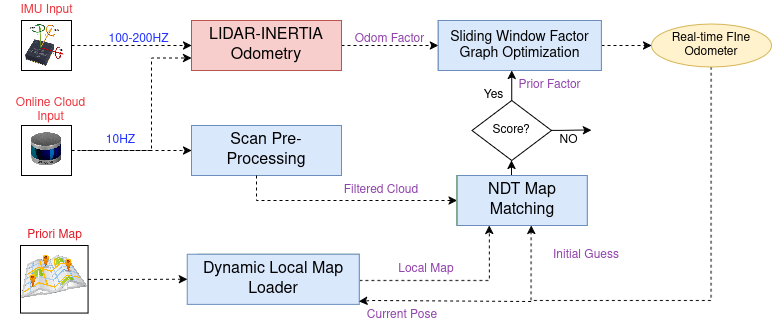
\includegraphics[width=1\linewidth]{images/system_overview.png}
    \caption{Complete Diagram of Map Based Localization}
    \label{fig:diagram-map-basedlocalization}
\end{figure}


\begin{algorithm}[H]
	\caption{LiDAR-Inertial Localization with Prior Map}
	\label{alg:localization-system}
	
	\textbf{Input:} $\mathcal{P}_t$ (LiDAR Point Cloud), $\mathcal{I}_t$ (IMU Data), $\mathcal{M}$ (Prior Map)\\
	\textbf{Output:} $\mathbf{T}_t$ (Real-time 6-DoF Pose)
	
	\begin{algorithmic}[1]
		
		\While{System is running}
		
		\State Acquire LiDAR point cloud $\mathcal{P}_t$ and IMU data $\mathcal{I}_t$
		
		\State Perform scan pre-processing on $\mathcal{P}_t$ to obtain filtered point cloud $\mathcal{P}_t^{filtered}$
		
		\State Estimate LiDAR-Inertial Odometry using $\{\mathcal{P}_t^{filtered}, \mathcal{I}_t\}$ to obtain odometry pose $\mathbf{T}_t^{lio}$	
		
		\If{$|| \mathbf{T}_t - \mathbf{T}_{last}^{map} || > d_{threshold}$}
		\State Load dynamic local map $\mathcal{M}_t^{local}$ from $\mathcal{M}$ centered at $\mathbf{T}_t^{lio}$
		\State Update $\mathbf{T}_{last}^{map} \gets \mathbf{T}_t$
		\EndIf
		
		\State Perform scan-to-map matching between $\mathcal{P}_t^{filtered}$ and $\mathcal{M}_t^{local}$ to obtain map-based pose $\mathbf{T}_t^{map}$
		
		\If{Matching score $> s_{threshold}$}
		\State Add prior factor with $\mathbf{T}_t^{map}$ to factor graph
		\EndIf
		
		\State Add odometry factor with $\mathbf{T}_t^{lio}$ to factor graph
		
		\State Optimize sliding window factor graph to obtain final pose $\mathbf{T}_t$
		
		\EndWhile
		
	\end{algorithmic}
\end{algorithm}


\subsection{LIDAR Scan Pre-Processing}
Before aligning each incoming LiDAR scan to the global map, we first subject the raw point cloud to a series of preprocessing operations. These operations improve both efficiency and reliability by filtering out irrelevant regions and outliers, downsampling to reduce data volume, and transforming the data into a consistent coordinate frame.Our approach, illustrated in Figure\ref{fig:lidar_scan_preprocessing}  consists of the following  main steps:
\begin{figure}
    \centering
    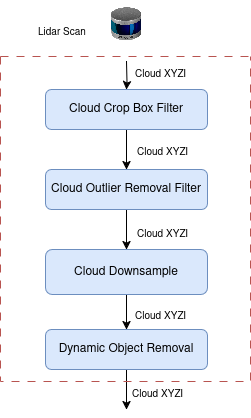
\includegraphics[width=0.4\linewidth]{images/LIDAR_PreProccess.drawio.png}
    \caption{LIDAR scan pre-processing}
    \label{fig:lidar_scan_preprocessing}
\end{figure}

\begin{itemize}
    \item \textbf{Crop-Box Filter}: This step confines the point cloud to a user-defined three-dimensional region (a bounding “box”) around the sensor or area of interest. By discarding all points lying outside this box, we focus only on the relevant portion of the scene, reducing both memory and computational overhead for subsequent processing.
    \item \textbf{Outlier Removal}: Once the point cloud is restricted to the area of interest, we remove random noise and spurious measurements using a statistical outlier filter. Concretely, we compute for each point the average distance to its k‐nearest neighbors. Points whose mean distance exceeds the global mean plus a chosen multiplier of the standard deviation are marked as outliers and deleted. This practice is a commonly adopted heuristic that discards stray or floating points, which might result from occasional sensor glitches or moving objects in the environment.
    \item \textbf{Voxel-Grid Downsampling} To further ease computational load, the point cloud is then downsampled. A typical approach uses a voxel-grid filter: space is subdivided into small volumetric “voxels,” and all points within each voxel are replaced by a single representative (often the centroid). This retains the main geometry while reducing point density, thereby speeding up map‐based matching algorithms.
    \item \textbf{Coordinate Transformation}:   Finally, we apply a rigid transformation that aligns the processed point cloud to a consistent coordinate frame used throughout our localization pipeline—the vehicle’s base link frame.This accounts for any known extrinsic offsets between the LiDAR sensor and the vehicle origin.
\end{itemize}

As summarized in Table~\ref{tab:lidar_preprocessing}, the LiDAR preprocessing parameters vary depending on the sensor type and application requirements. All filtering and scan processing operations are implemented using the Point Cloud Library (PCL).



\begin{table}[htbp]
\centering
\caption{LiDAR Scan Processing Methods and Parametrs  Across Different Sensor Setups}
\label{tab:lidar_preprocessing}
\begin{tabular}{|p{3.5cm}|p{3.5cm}|p{3.5cm}|p{3.5cm}|}
\hline
\textbf{Processing Step} & \textbf{KITTI(Velodyne HDL-64E)} & \textbf{MulRan(Ouster-OS1-64)} & \textbf{(Ouster-OS1-128)} \\
\hline
LiDAR Type & Velodyne HDL-64E & Ouster OS1-64 & Ouster OS1-128 \\
% \hline
% \textbf{Vertical Channels} & 64 & 64 & 128 \\
% \hline
% \textbf{Vertical FOV} & $\pm$2° to $\pm$24.8° ($\sim$26.8° total) & $\pm$16.6° ($\sim$33.2° total) & $\pm$22.5° ($\sim$45° total) \\
\hline
Max Range & $\sim$120 m & $\sim$120 m & $\sim$240 m \\
\hline
Crop Box Filter & 90-100m & 90-100m & 180-200m\\
\hline
Downsampling Method & Voxel-Grid(leaf-size: 0.5m) & Voxel-Grid(leaf-size: 0.4-0.6 m) & Voxel-Voxel(0.5-0.8 m) \\
\hline
Outlier Removal & Statistical (K=50, Std=1.0) & Statistical (K=40, Std=1.0) & Statistical(K=40 ,Std=1,0) \\
\hline
% \textbf{Ground Removal} & Not used & Yes — flat surface segmentation &  Yes — flat surface segmentation \\
% \hline
\end{tabular}
\end{table}

\subsection{Map Pre-Processing}

\subsubsection{Grid-based Map Point Cloud Division }

When using a high-resolution point cloud map for localization in large areas, loading the entire map can overwhelm memory and computation. To tackle this, \emph{we divide the global map} into smaller ``tiles,'' each containing only part of the overall data as shown in \ref{fig:pointcloud division}. Below is a brief outline:

\begin{itemize}
    \item \textbf{Rationale}: Instead of loading the entire map, the localization system can dynamically fetch only the sub-map (tile) around the vehicle's estimated position, saving memory and speeding up matching.
    \item \textbf{Grid Definition}: A user-chosen tile size (e.g., 100\,m\,$\times$\,100\,m) defines a regular grid overlay on the map's bounding box. Each tile's data are saved as a separate file.
    \item \textbf{Offline Preparation}: This division happens once, offline. The resulting sub-map files (e.g., \texttt{tile\_0\_0.pcd}, \texttt{tile\_1\_0.pcd}) are stored on disk.
    \item \textbf{Tile Indexing}: A simple coordinate scheme (e.g., $(i, j)$ for each tile) allows quick lookup. As the vehicle moves, the system checks its approximate position and loads only the necessary tiles.
\end{itemize}

\begin{figure}
    \centering
    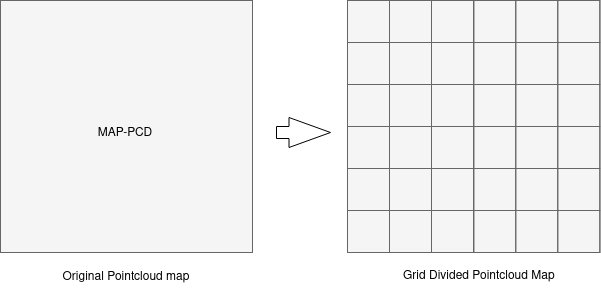
\includegraphics[width=0.8
    \linewidth]{images/map.drawio.png}
    \caption{Grid Based Point-cloud division }
    \label{fig:pointcloud division}
\end{figure}
\subsection{Dynamic Map Loading}

Even with a divided map, loading all tiles at once is inefficient. Therefore, the system adopts a \emph{dynamic loading} strategy, where only the sub-clouds near the robot's current position are fetched in real time. Concretely:

\begin{itemize}
    \item \textbf{Robot Pose Check}: At each iteration (or after the robot travels a threshold distance), the system retrieves the robot's latest pose estimate.
    \item \textbf{Loading Radius}: Based on sensor range (e.g., LiDAR maximum range) and a user-defined margin, we determine a radius (e.g., 80\,m) around the current pose within which map data is required.
    \item \textbf{Partial Tile Retrieval}: Only tiles intersecting this radius are loaded, reducing memory overhead. As the robot moves and crosses tile boundaries, newly relevant tiles are loaded and old ones are freed.
    \item \textbf{Update Frequency}: To avoid frequent reloads, the system triggers map updates only after the robot has moved a certain threshold (e.g., 20\,m) since the last update.
\end{itemize}

This on-demand \emph{dynamic loading} ensures that the system retains sufficient map detail for accurate localization while minimizing both I/O and memory consumption. 

\subsection{LIDAR Inertia Odometry}

\subsection{Scan-to-Map Matching}

\subsubsection{}





